\documentclass[a4paper,11.5pt]{article}
\usepackage[textwidth=170mm, textheight=230mm, inner=20mm, top=20mm, bottom=30mm]{geometry}
\usepackage[normalem]{ulem}
\usepackage[utf8]{inputenc}
\usepackage[T1]{fontenc}
\PassOptionsToPackage{defaults=hu-min}{magyar.ldf}
\usepackage[magyar]{babel}
\usepackage{amsmath, amsthm,amssymb,paralist,array, ellipsis, graphicx, float}
%\usepackage{marvosym}

\makeatletter
\renewcommand*{\mathellipsis}{%
	\mathinner{%
		\kern\ellipsisbeforegap%
		{\ldotp}\kern\ellipsisgap%
		{\ldotp}\kern\ellipsisgap%
		{\ldotp}\kern\ellipsisaftergap%
	}%
}
\renewcommand*{\dotsb@}{%
	\mathinner{%
		\kern\ellipsisbeforegap%
		{\cdotp}\kern\ellipsisgap%
		{\cdotp}\kern\ellipsisgap%
		{\cdotp}\kern\ellipsisaftergap%
	}%
}
\renewcommand*{\@cdots}{%
	\mathinner{%
		\kern\ellipsisbeforegap%
		{\cdotp}\kern\ellipsisgap%
		{\cdotp}\kern\ellipsisgap%
		{\cdotp}\kern\ellipsisaftergap%
	}%
}
\renewcommand*{\ellipsis@default}{%
	\ellipsis@before
	\kern\ellipsisbeforegap
	.\kern\ellipsisgap
	.\kern\ellipsisgap
	.\kern\ellipsisgap
	\ellipsis@after\relax}
\renewcommand*{\ellipsis@centered}{%
	\ellipsis@before
	\kern\ellipsisbeforegap
	.\kern\ellipsisgap
	.\kern\ellipsisgap
	.\kern\ellipsisaftergap
	\ellipsis@after\relax}
\AtBeginDocument{%
	\DeclareRobustCommand*{\dots}{%
		\ifmmode\@xp\mdots@\else\@xp\textellipsis\fi}}
\def\ellipsisgap{.1em}
\def\ellipsisbeforegap{.05em}
\def\ellipsisaftergap{.05em}
\makeatother

\usepackage{hyperref}
\hypersetup{
	colorlinks = true	
}

\begin{document}
	%%%%%%%%%%%RÖVIDÍTÉSEK%%%%%%%%%%
	\setlength\parindent{0pt}
	\def\a{\textbf{a}}
	\def\b{\textbf{b}}
	\def\N{\hskip 10 true mm}
	\def\a{\textbf{a}}
	\def\b{\textbf{b}}
	\def\c{\textbf{c}}
	\def\d{\textbf{d}}
	\def\e{\textbf{e}}
	\def\gg{$\gamma$}
	\def\vi{\textbf{i}}
	\def\jj{\textbf{j}}
	\def\kk{\textbf{k}}
	\def\fh{\overrightarrow}
	\def\l{\lambda}
	\def\m{\mu}
	\def\v{\textbf{v}}
	\def\0{\textbf{0}}
	\def\s{\hspace{0.2mm}\vphantom{\beta}}
	\def\Z{\mathbb{Z}}
	\def\Q{\mathbb{Q}}
	\def\R{\mathbb{R}}
	\def\C{\mathbb{C}}
	\def\N{\mathbb{N}}
	\def\Rn{\mathbb{R}^{n}}
	\def\Ra{\overline{\mathbb{R}}}
	\def\sume{\displaystyle\sum_{n=1}^{+\infty}}
	\def\sumn{\displaystyle\sum_{n=0}^{+\infty}}
	\def\biz{\emph{Bizonyítás:\ }}
	\def\narrow{\underset{n\rightarrow+\infty}{\longrightarrow}}
	\def\limn{\displaystyle\lim_{n\to +\infty}}
	%\def\definition{\textbf{Definíció:\ }}
	%\def\theorem{\textbf{Tétel:\ }}
	%\def\note{\emph{Megjegyzés:\ }}
	%\def\example{\textbf{Példa:\ }} 
	
	\theoremstyle{definition}
	\newtheorem{theorem}{Tétel}[subsection] % reset theorem numbering for each chapter
	
	\theoremstyle{definition}
	\newtheorem{definition}[theorem]{Definíció} % definition numbers are dependent on theorem numbers
	\newtheorem{example}[theorem]{Példa} % same for example numbers
	\newtheorem{note}[theorem]{Megjegyzés} % same for example numbers
	%%%%%%%%%%%%%%%%%%%%%%%%%%%%%%%%%
	\begin{center}
		{\LARGE \textbf{Analízis II}}
		
		{\large \textbf{Előadás jegyzet}}
		
		1. óra
	\end{center}
	A jegyzetet \textsc{Umann} Kristóf készítette Dr. \textsc{Szili} László előadásán. (\today)
	
	Külön köszönet jár \textsc{Csonka} Szilviának a képek elkészítésért.
	\bigskip
	
	Tantárgyi honlap: \url{http://numanal.inf.elte.hu/~szili/Oktatas/An2_BSc_2016/index_An2_2016.htm}
	
	\begin{center}
		\section{Követelményrendszer:}
	\end{center}
		\begin{compactitem}
			\item Heti rendszeres számonkérés
			\item megajánlott
			\item kötelező előadásra járás (12:15kor kezdés)
			\item gyakorlati jegy kell (aminek anyaga már a honlapon kint van)
		\end{compactitem}
		\begin{center}
			\section{\textbf{Függvények folytonossága}}
		\end{center}
	\subsection{Szemléletes jelentése:}
		\begin{figure}[!h]
			\centering
			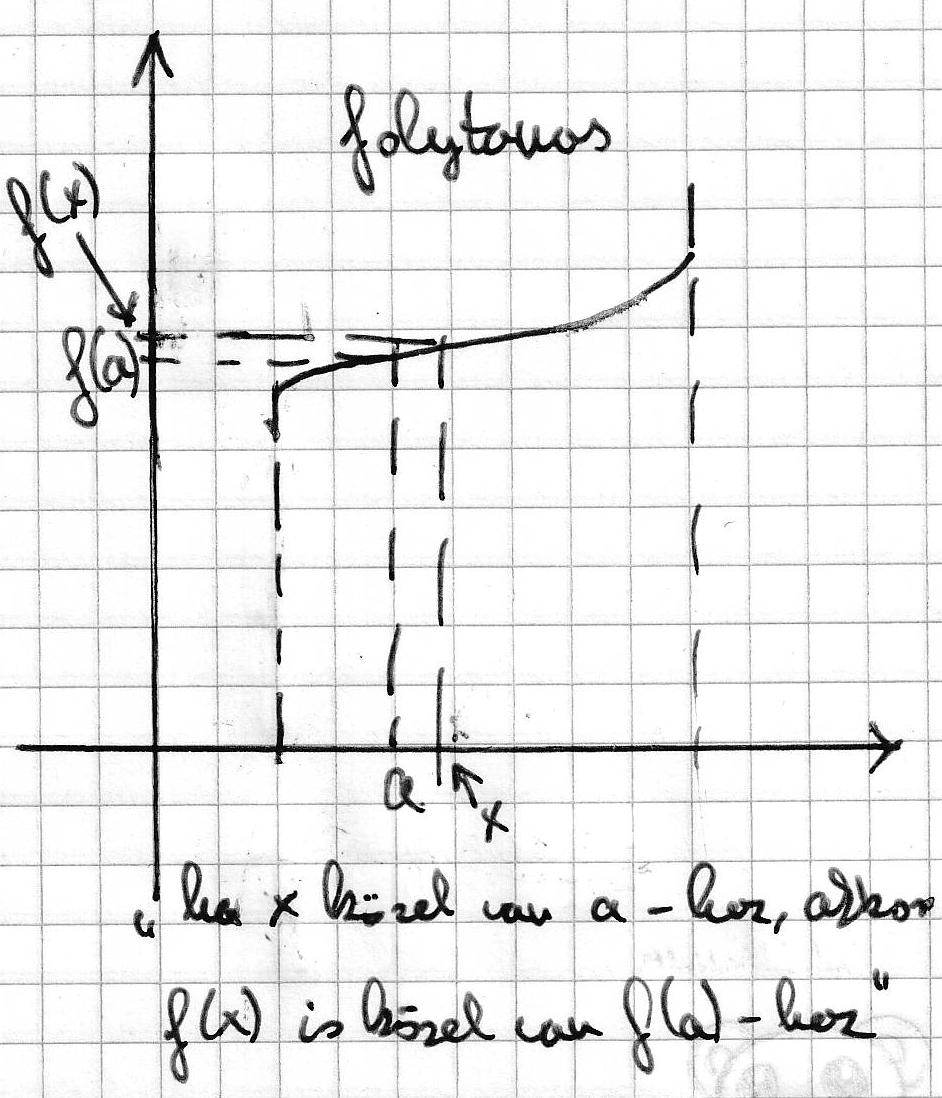
\includegraphics[height=5cm]{kepek/1_abra_folytonos.jpg}\quad \quad 
			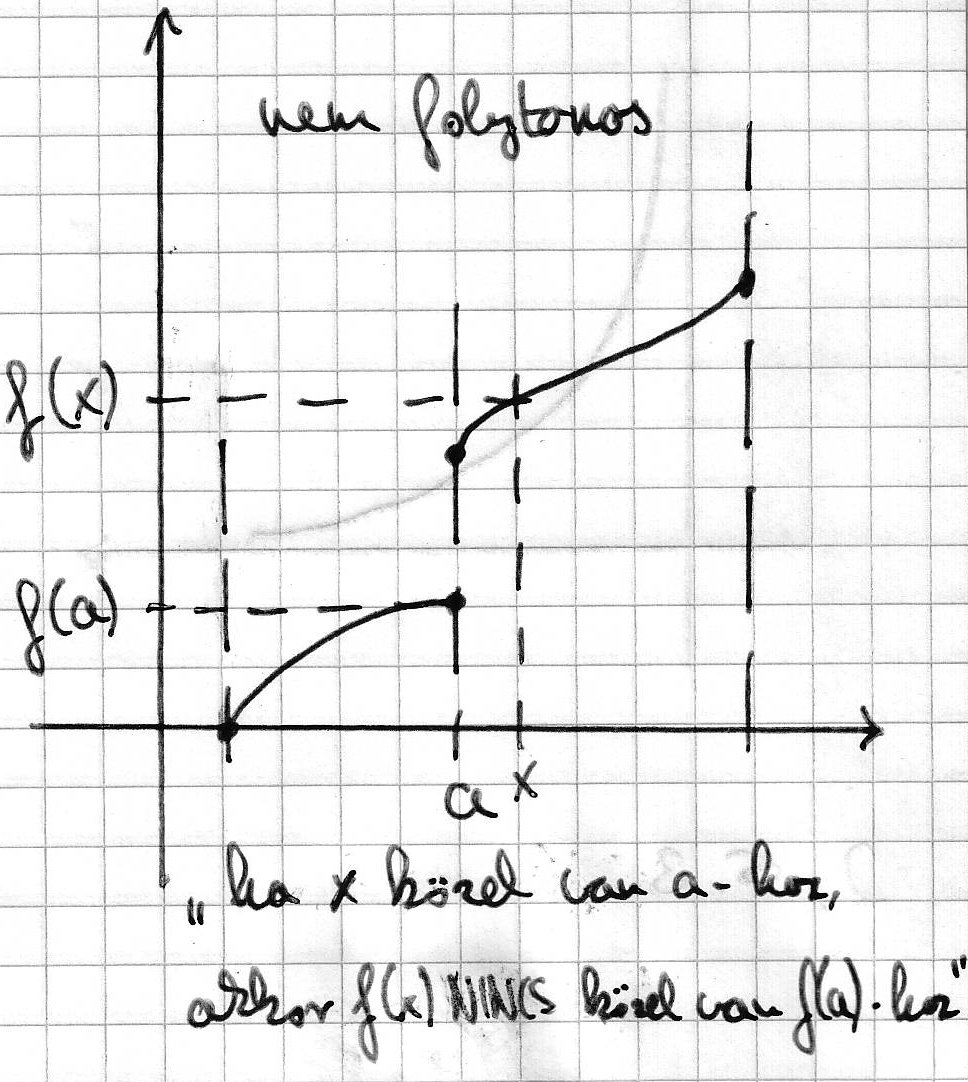
\includegraphics[height=5cm]{kepek/1_abra_nemfolytonos.jpg}
			\caption{Nem folytonos, ''ha $x\sim a$-hoz akkor $f(x)$ nincs közel $f(a)$-hoz''.}\label{fig_nemfolytonos}
		\end{figure}
		
		\begin{note}
			Hasonló probléma: fv. határértéke (végesben vett véges h.é.)
			\[a, A\in \R,\quad f\in\R\to\R,\quad a\in\mathcal{D}'_f \]
			\[\displaystyle\lim_af=A \quad \Leftrightarrow \quad 
			\left\{
			\begin{gathered}
			\forall \varepsilon >0,\quad  \exists \sigma>0,\quad  \forall x \in \mathcal{D}_f \\
			0<|x-a|<\sigma \quad \text{esetén} \quad|f(x)-A| < \varepsilon
			\end{gathered}\right. \]
			azaz, ha ,,$x\sim a$, akkor $f(x) \sim A$.
		\end{note}
		
	\subsection{\textbf{Pontbéli folytonosság}}
		\begin{definition}
			Az $f\in \R\to\R$ fv az $a\in\mathcal{D}_f$ pontban folytonos, ha
			\[ \forall \varepsilon>0 \quad \exists \delta>0, \quad \forall x \in \mathcal{D}_f:\quad  |x-a|<\delta, \quad |f(x)-f(a)|<\varepsilon \]
			Jelölése: $f\in C(a)$.
		\end{definition}
		
		\begin{note} \
			
			\begin{enumerate}
				\item Csak ÉT-beli pontban ért. a folytonosság
				\item Személetes jelentése ,,ha $x\sim a \Rightarrow f(x) \sim f(a)$''
			\end{enumerate}
		\end{note}
		
		\begin{example} 
			$f(x) :=\text{sign(x)}\quad (x\in\R)$
			
			\begin{figure}[H]
				\centering
				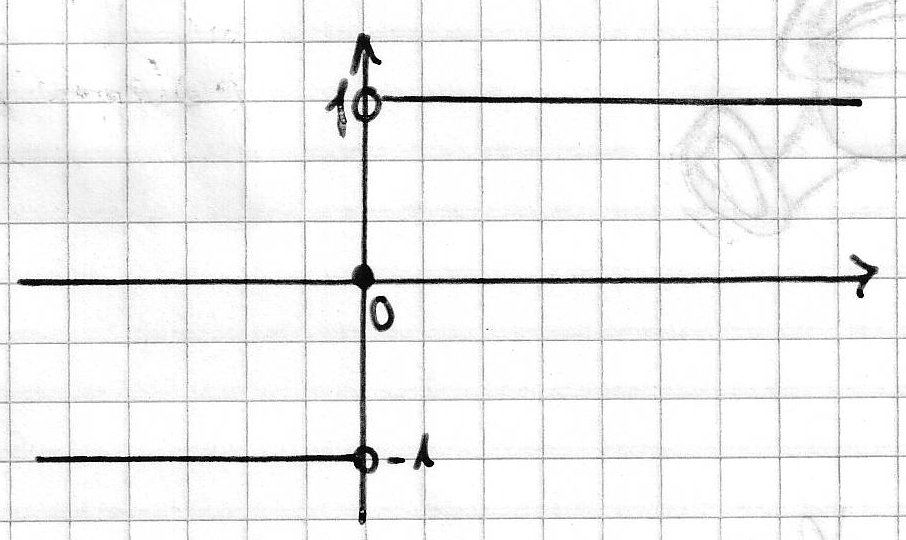
\includegraphics[height=3cm]{kepek/2_abra_signum.jpg}\quad \quad \quad 
				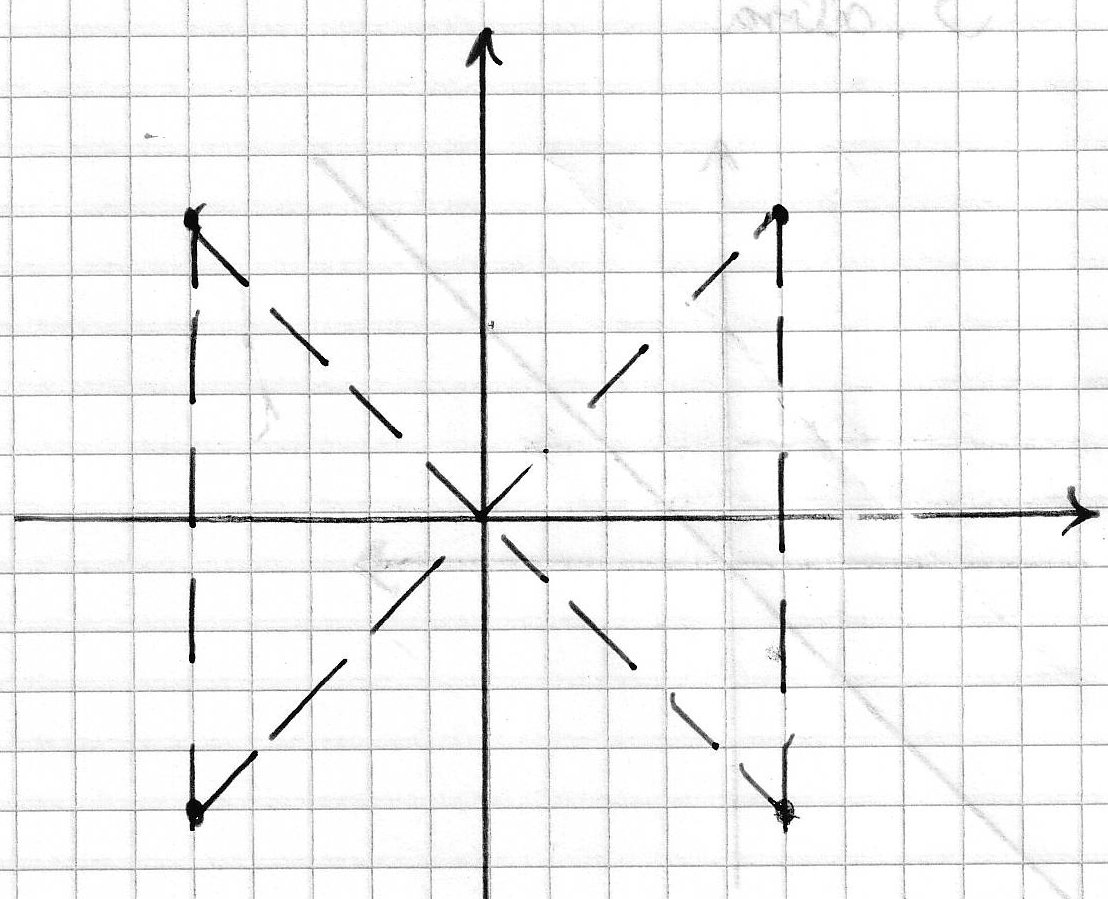
\includegraphics[height=3cm]{kepek/2_abra_dirichlet.jpg}
				\caption{sign$(x)$ és a Dirichlet függvény}\label{fig_dirichlet}
			\end{figure}
			
			$f\notin C\{0\},$ \quad ui.\quad $ \exists\varepsilon > 0 \quad \forall \delta > 0 \quad \exists |x|<\delta: \quad |f(x)-0|\geq\varepsilon$.
			
		\end{example} 
		
		\begin{example}
			Dirichlet fv.
			$f(x)=
			\left\{\begin{gathered}
				x \in \Q \\
				-x \in \Q^*
			\end{gathered}\right.$\quad \quad 
			Ekkor: $\left\{\begin{gathered}
				f\in C\{0\}\\
				f \notin C\{a\} \text{ \quad ha \quad }  a\in\R\backslash\{0\}
			\end{gathered} \right.$
		\end{example}
		
		\begin{theorem}
			Ha $a\in\mathcal{D}_f$ izolált pont (azaz $\exists K(a): K(a) \cap\mathcal{D}_f = \{a\}) \quad \Rightarrow \quad f\in C\{a\}$
			
			Biz: $\checkmark \quad \blacksquare$
		\end{theorem} 
		\medskip
		
		\begin{theorem}
			(A folyt. és határérték kapcsolata)
		
		Ha $a\in \mathcal{D}_f\cap\mathcal{D}'_f,$ akkor 
		\[f\in C\{a\} \quad \Leftrightarrow\quad  \exists \lim_af \text{ és }\lim_af=f(a).  \]
		
		Biz: \checkmark\quad $\blacksquare$
		
		\end{theorem}
		
		\begin{theorem}
			Hatványsor összegfüggvénye a konvergenciahalmaz minden
			\begin{enumerate}
				\item pontjában folytonos
				\item Az $\exp, \sin, \cos,$ sh, ch, $\forall \R$-beli pontban folytonos.
				$\blacksquare$
			\end{enumerate}
		
		\end{theorem}
		\begin{theorem}
			(Folytonosságra vonatkozó átviteli elv)
			
			Tegyük fel, hogy $f\in\R\to\R;\quad  a\in\mathcal{D}_f$.
			
			\[ f\in C\{a\}\quad \Leftrightarrow\quad  \forall(x_n):  \N\to\mathcal{D}_f,\quad  \lim(x_n) = a \]
			esetén
			
			\[ \limn f(x_n) = f(a). \]
			
			Bizonyítás: 
			\begin{itemize}
				\item Ha $a\in\mathcal{D}_f\cap\mathcal{D'}_f,$ akkor \checkmark
				\item Ha $a\in\mathcal{D}_f$ és $a\notin \mathcal{D'}_f \Rightarrow a$ izolált pont. $\blacksquare$
			\end{itemize}
			
		\end{theorem}
		\begin{theorem}
			(Műveletek és folytonosság)

			Tegyük fel, hogy $f,g\in\R\to\R, \quad f,g\in C\{a\}.$ Ekkor 
			\begin{enumerate}
				\item $\lambda f,\quad  f+g, \quad f\cdot g,\quad  \frac{f}{g} \quad (g(a)\not=0) \quad \in C\{a\}.$ \quad ($\lambda \in \R\ $tetszőleges)
				\item Ha $\mathcal{R}_g\subset\mathcal{D}_f, \quad g\in C\{a\}, \quad f\in C\{g(a)\}\quad \Rightarrow\quad  f\circ g\in C\{a\}$
			\end{enumerate}
			Bizonyítás: Műveleti tételek. \quad $\blacksquare$
		\end{theorem}
		
	\subsection{\textbf{Egyoldali folytonosság}}
		
		\begin{definition}
			Legyen $f\in\R\to\R$ és $a\in\mathcal{D}_f$. Az $f$ függvény  jobbról folytonos $a$-ban, ha
		
			\[\forall \varepsilon>0, \quad \exists \delta>0,\quad  \forall x\in\mathcal{D}_f,\quad  a\leq x< a + \delta \text{ \quad esetén\quad  } |f(x)-f(a)|<\varepsilon  \]
		\end{definition}
		\begin{note}
			Balról folyt. hasonló
		\end{note}
		\begin{theorem}
			$f\in C\{a\} \Leftrightarrow$ ha jobbról és balról is folytonos.
		\end{theorem}
		
	\subsection{\textbf{Halmazon folytonos függvények.}}
	
		\begin{definition}
			Legyen $f\in\R\to\R,\quad  A\subset\mathcal{D}_f.$ Az $f$ fv. folytonos az $A$ halmazon, ha 
			\[ \forall a\in A\text{ \quad esetén\quad  } f\big|_A \in C\{a\}.\]
			
			Jelölése: $f\in C(A)$
		\end{definition}
		
		\begin{note}
			Müvelete tételek halmazon folytonos függvényekre is érvényesek.
		\end{note}
	\subsection{Korlátos és zárt $[a,b]$ intervallumon folytonos függvények tulajdonságai}
		(végig: $-\infty <a<b<+\infty$, un. kompakt intervallum)
	
		\begin{theorem}
			($[a,b]$ folytonos függvény korlátos)
		
			Tegyük fel, hogy 
			$\left.
			\begin{gathered}
				f:[a,b]\to\R \\
				\text{folytonos } [a,b]\text{-n}
			\end{gathered}
			\right\}\quad  \Rightarrow \quad f $ korlátos.
			\begin{note}\ 
				
				\begin{figure}[!h]
					\centering
					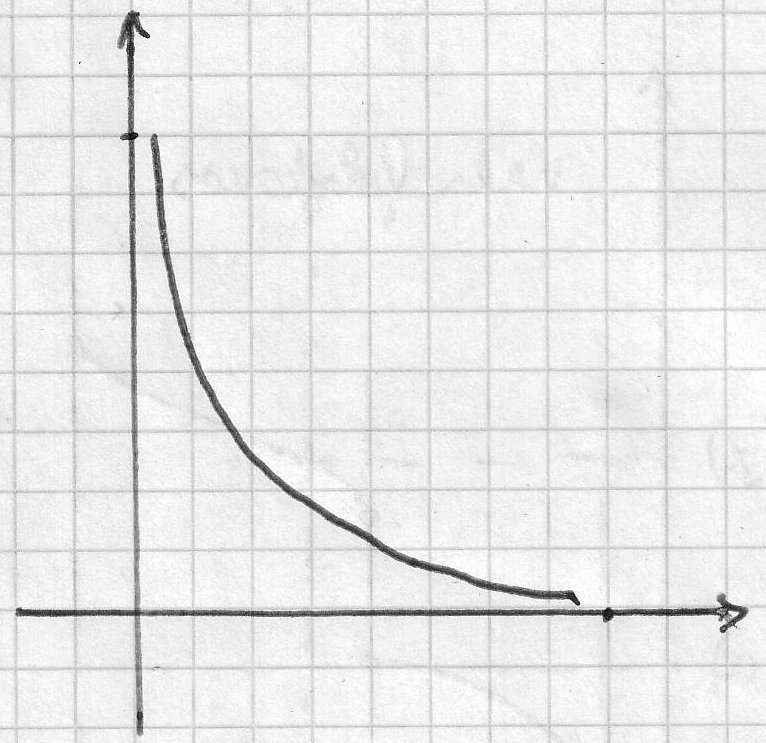
\includegraphics[height=3cm]{kepek/3_abra.jpg}
					\caption{Folytonos, de nem korlátos!}\label{fig_3}
				\end{figure}
			\end{note}
			
			
			Bizonyítás: $f$ korlátos, ha
			\[ \exists K>0, \quad \forall x \in [a,b]: \quad |f(x)|\leq K \]
			Indirekt: Tegyük fel, hogy nem korlátos, azaz, 
			
			\begin{gather}
				\forall K>0, \quad \exists x \in [a,b]: \quad |f(x)|> K \notag\\
				\Rightarrow \forall n = 1,2 \quad \exists x_n \in [a,b], \quad |f(x_n)|\geq n\label{reference} 
			\end{gather} 
			
			Tehát: $(x_n)\subset[a,b]$ korlátos sorozat $\overset{\text{B-W kiv.}}{\underset{\text{tétel}}{\Longrightarrow}} \exists (x_{n_k})$ konv. részsorozat. 
			
			Legyen
			\[ \alpha:=\lim(x_{n_k}) \]
			Ekkor: $\alpha\in[a,b]$.\quad
			
			(Indirekt: Tegyük fel, hogy $\alpha \notin [a,b] \quad \Rightarrow \quad \exists K (\alpha) \cap[a,b] = \emptyset$.
			
			$\alpha:=\lim(x_{n_k})\quad  \Rightarrow \quad \exists k_0\in\N,\quad \forall k\geqq k_0, \quad x_{n_k}\in K(\alpha).$ 
			Ez ellentmondás, ui. $x_{n_k}\in[a,b])$.
			\medskip
			
			Az $f$ folytonos $[a,b]$-n $\Rightarrow $
			\[ f\in C \{\alpha\}\quad \overset{\text{átviteli elv}}{\Rightarrow} \quad x_{n_k} \to \alpha \quad \Rightarrow\quad  f(x_{n_k}) \to f(\alpha)\quad  \Rightarrow \quad \left(f(x_{n_k})\right) \quad \text{korlátos, mert konv.}\]
			
			Ez ellentmond \ref{reference}-nek.\quad $\blacksquare$
			
		\end{theorem}
		
		\begin{definition}
			Az $f\in\R\to\R$ fv-nek van \textit{abszolút} (vagy \textit{globális}) \textit{maximuma}, ha 
			\[ \exists \alpha\in\mathcal{D}_f: \quad \forall x\in\mathcal{D}_f: \quad f(x)\leqq f(\alpha) \]
			
			$\alpha$: \textit{absz. maximum hely}
			
			$f(\alpha)$: a fv. \textit{absz. maximuma}.
		\end{definition}
		
		\begin{note}
			Abszolút minimum hasonló.
		\end{note}
		\begin{note}
			Abszolút szélső érték: abszolút max. vagy abszolút min.
		\end{note}
		
		\begin{example}
			$f(x) =\displaystyle  \frac{1}{x} \quad (x\in (0,1))$
			
			\begin{figure}[H]
				\centering
				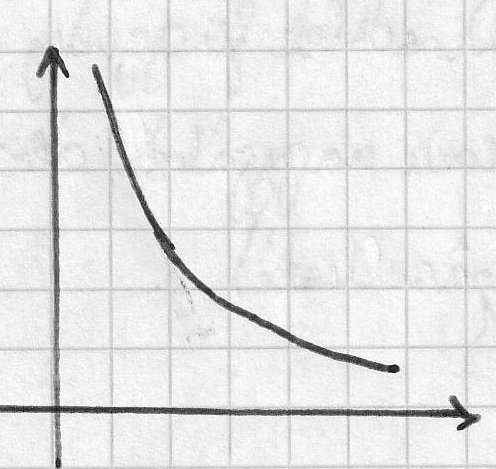
\includegraphics[height=3cm]{kepek/4_abra.jpg}
				\caption{Folytonos, NINCS szélső értéke.}\label{fig_4}
			\end{figure}
		\end{example}
		
		\begin{example}
			$f(x) = x$
			
			\begin{figure}[!h]
				\centering
				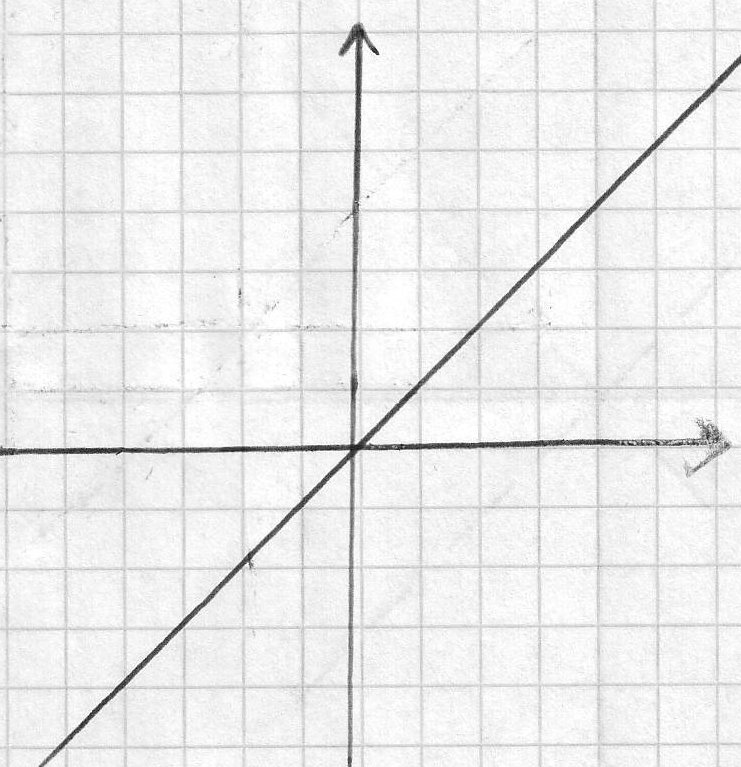
\includegraphics[height=3cm]{kepek/5_abra.jpg}
				\caption{Folytonos, NINCS szélső értéke.}\label{fig_5}
			\end{figure}
			
		\end{example}
		
		\begin{example}\
			
			 \begin{figure}[!h]
			 	\centering
			 	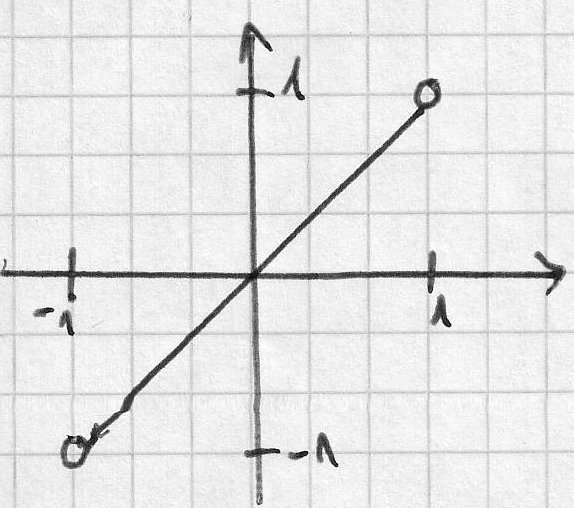
\includegraphics[height=3cm]{kepek/6_abra.jpg}
			 	\caption{Nem folytonos, nincs szélső értéke.}\label{fig_6}
			 \end{figure}
			
			
		\end{example}
		
		\begin{note}
			Azonban: $[a,b]$-n folytonos fv-nek van absz. sz.é.-e.
		\end{note}
		
		\begin{theorem}
			(Weierstrass)
			
			Tegyük fel, hogy:
			\[ \left.
			\begin{gathered} 
				f: [a,b]\to\R \\
				\text{folytonos } [a,b] 
			\end{gathered}
			\right\} \Rightarrow
			\begin{gathered}
				\text{$f$-nek $\exists$ absz. szélsőértéke, azaz\quad }\exists \alpha, \beta, \in [a,b]: \\
				f(x) \leq f(\alpha) \\
				f(\beta) \leq f(x)
			\end{gathered}\quad (x\in[a,b])\]
			
			Biz: $f$ folytonos $[a,b]$-n $\Rightarrow f$ korlátos.
			
			Ekkor:\[
			\begin{gathered}
			\exists \sup\{f(x)\ |\ x\in [a,b]\} =: M \in \R\\
			\exists \inf\{f(x)\ |\ x\in [a,b]\} =: m \in \R\\
			\end{gathered}\]
			Igazoljuk: $\exists \alpha \in [a,b]:\quad  f(\alpha) = M$.
			
			\begin{gather}
			M \sup\quad  \Rightarrow \quad \forall n \in \N,\quad  \exists y_n\in\mathcal{R}_f:\quad  M - \frac{1}{n} < y_n \leq M 
			\label{weierstrass-label}
			\end{gather}
			Viszont: \[y_n\in\mathcal{R}_f \quad \Rightarrow\quad  \exists x_n\in [a,b]:\quad  f(x_n) = y_n,\quad (\forall n\in\N)\]
			
			Az $(x_n): \N\to[a,b]$ korlátos sorozat $\quad \overset{\text{B-W kiv.}}{\underset{\text{tétel}}{\Longrightarrow}} \quad \exists (x_{n_k})$ konvergens részsorozata.
			
			Legyen $\lim(x_{n_k}) =: \alpha \in [a,b]$ (indirekt)
			
			\[f\text{ folyt. }[a,b]\text{-n }\quad \Rightarrow \quad f\in C\{\alpha\} \quad \overset{\text{átviteli elv}}{\Rightarrow}\quad 
			\lim\underbrace{f (x_{n_k})}_{y_{n_k}} = f(\alpha)\]
			\[ \limn y_{n_k} = f(\alpha) \quad \Rightarrow\quad M = f(\alpha) \]
			Ez ellentmondás. (lásd: \ref{weierstrass-label})\quad $\blacksquare$
		\end{theorem}
\end{document}